% Snowflake Data Engineering — Chapter 3 | original manuscript draft
% Author: Arman Golbidi | Editorial snapshot: 21 October 2026
% Compile: xelatex -interaction=nonstopmode -halt-on-error Snowflake_Data_Engineering_Chapter_03.tex
% Trim: 178 x 254 mm; margins inside 23 mm / outside 17 mm / top-bottom 19 mm.
% Body: 10.75 pt / 13.65 pt leading = 1.27 line-height ratio; code: 8.75 pt.
\documentclass[11pt,twoside]{article}
\usepackage[paperwidth=178mm,paperheight=254mm,inner=23mm,outer=17mm,top=19mm,bottom=19mm,headheight=5mm,headsep=4mm,footskip=9mm]{geometry}
\usepackage{fontspec}
\setmainfont{LibertinusSerif-Regular.otf}[BoldFont=LibertinusSerif-Bold.otf,ItalicFont=LibertinusSerif-Italic.otf,BoldItalicFont=LibertinusSerif-BoldItalic.otf]
\setsansfont{LibertinusSans-Regular.otf}[BoldFont=LibertinusSans-Bold.otf,ItalicFont=LibertinusSans-Italic.otf]
\setmonofont{LibertinusMono-Regular.otf}[Scale=0.91]
\usepackage[english]{babel}
\usepackage{microtype}
\usepackage{setspace}
\setstretch{1.0}
\usepackage{titlesec,enumitem,tabularx,array,booktabs,needspace,fancyhdr,lastpage}
\usepackage[most]{tcolorbox}
\usepackage{tikz}
\usetikzlibrary{arrows.meta,positioning,fit,shapes.misc,calc}
\usepackage{listings}
\usepackage{xcolor}
\usepackage{hyperref}
\hypersetup{colorlinks=true,urlcolor=steelblue,linkcolor=steelblue,pdfauthor={Arman Golbidi},pdftitle={Snowflake Data Engineering - Chapter 3: Setting Up Snowflake and Development Environments},pdfsubject={English technical book manuscript, third chapter, 178 x 254 mm}}
\definecolor{navy}{HTML}{15334A}
\definecolor{steelblue}{HTML}{17779B}
\definecolor{teal}{HTML}{12888A}
\definecolor{lightblue}{HTML}{ECF5F7}
\definecolor{papergray}{HTML}{F2F5F6}
\definecolor{inkgray}{HTML}{4A5862}
\definecolor{thinrule}{HTML}{CBD7DB}
\AtBeginDocument{\color{navy}\fontsize{10.75}{13.65}\selectfont}
\setlength{\parindent}{0pt}
\setlength{\parskip}{3.3pt plus 0.7pt minus 0.6pt}
\setlist[itemize]{leftmargin=4mm,itemsep=1pt,topsep=2pt,parsep=0pt}
\setlist[enumerate]{leftmargin=5mm,itemsep=1pt,topsep=2pt}
\titleformat{\section}{\sffamily\bfseries\color{navy}\fontsize{14}{17}\selectfont}{}{0pt}{}
\titlespacing*{\section}{0pt}{8pt}{4pt}
\titleformat{\subsection}{\sffamily\bfseries\color{steelblue}\fontsize{10.8}{13}\selectfont}{}{0pt}{}
\titlespacing*{\subsection}{0pt}{5pt}{1pt}
\newcommand{\topic}[2]{\subsection*{#1\quad #2}}
\newcommand{\repo}[2]{\par\begingroup\fontsize{8.0}{9.6}\selectfont\sffamily\color{inkgray}\textbf{Project reference:} \href{#2}{#1}. \textit{Not independently executed; rights review pending.}\par\endgroup}
\newtcolorbox{insight}[1][]{enhanced,breakable,colback=lightblue,colframe=thinrule,boxrule=.45pt,arc=1.3mm,left=2.8mm,right=2.8mm,top=1.8mm,bottom=1.8mm,before skip=5pt,after skip=5pt,#1}
\newtcolorbox{whitebox}[1][]{enhanced,breakable,colback=papergray,colframe=thinrule,boxrule=.35pt,arc=1mm,left=2.6mm,right=2.6mm,top=1.5mm,bottom=1.5mm,before skip=4pt,after skip=5pt,#1}
\lstdefinestyle{chaptercode}{basicstyle=\ttfamily\fontsize{8.75}{10.7}\selectfont,backgroundcolor=\color{papergray},frame=single,framerule=.35pt,rulecolor=\color{thinrule},breaklines=true,columns=fullflexible,keepspaces=true,showstringspaces=false,aboveskip=5pt,belowskip=5pt,xleftmargin=2mm,xrightmargin=1mm,framexleftmargin=2mm,framexrightmargin=1mm}
\lstset{style=chaptercode}
\pagestyle{fancy}
\fancyhf{}
\fancyhead[LE]{\sffamily\fontsize{7.6}{9}\selectfont\color{inkgray}\textsc{Snowflake Data Engineering}}
\fancyhead[RO]{\sffamily\fontsize{7.6}{9}\selectfont\color{inkgray}\textsc{03 / Development Environments}}
\fancyfoot[LE,RO]{\sffamily\bfseries\fontsize{8.2}{9}\selectfont\color{steelblue}\thepage}
\fancyfoot[LO,RE]{\sffamily\fontsize{7.6}{9}\selectfont\color{inkgray}Arman Golbidi \quad | \quad Chapter 03}
\renewcommand{\headrulewidth}{0.35pt}
\renewcommand{\footrulewidth}{0pt}
\setcounter{page}{39}
\raggedbottom

% CHAPTER 02 ONLY, pages 39--56 in the planned book
\begin{document}
% PAGE 39 / Chapter opener
{\sffamily\bfseries\color{teal}\fontsize{10}{12}\selectfont CHAPTER 03\quad /\quad DEVELOPMENT ENVIRONMENTS}\par\vspace{2mm}
{\sffamily\bfseries\color{navy}\fontsize{23}{26}\selectfont Setting Up Snowflake\par and Development\par Environments}\par
\vspace{1.6mm}{\color{steelblue}\rule{\linewidth}{1.5pt}}\par\vspace{2mm}
{\sffamily\color{inkgray}\fontsize{11.2}{15}\selectfont A safe first environment is a design decision, not an administrative afterthought.}\par\vspace{2mm}

It is Friday afternoon. An engineer has a promising energy dashboard and wants to test one more transformation before sharing it with colleagues. The fastest option appears to be an unrestricted account, a warehouse that never suspends, and SQL copied directly into a browser worksheet. The demonstration works. On Monday, however, nobody can explain who owns the tables, how much the experiment cost, why a colleague can change the raw data, or which version of the SQL created the results.

The mistake was not a missing Snowflake feature. The team had built a \emph{working query} without building a \emph{repeatable environment}. This chapter establishes a small, inspectable workspace for the Finland Energy Analytics project. We shall separate administration from everyday use; treat credentials as secrets; make data objects predictable; and design clean teardown before the first chargeable query.

\begin{insight}
\textbf{The design question}\par
How can another engineer reconstruct our environment, run only the work they are authorized to run, establish that it behaves correctly, and shut it down without risking production data or uncontrolled charges?
\end{insight}
\textbf{By the end of this chapter you will be able to:}
\begin{itemize}
\item distinguish organizations, accounts, editions, regions, and trial limits;
\item navigate Snowsight and record reproducible session evidence;
\item provision an X-Small test warehouse, database, schema, and small sample table;
\item grant least-privilege reader access and verify a denied operation;
\item connect Snowflake CLI and Python without committing passwords;
\item distinguish budgets from warehouse resource monitors; and
\item produce reviewable bootstrap, verification, and cleanup artifacts.
\end{itemize}
\textbf{Prerequisites.} Chapters 1--2 and elementary SQL. A Snowflake account is optional for the \emph{offline} design exercises; execution of cloud SQL requires an authorized account, billable credits or trial allowance, and a suitably privileged administrator. All displayed cloud outputs are \emph{expected examples}, not claims of a live run.

\newpage
% PAGE 40 / 3.1
\section*{3.1\quad Accounts, organizations, editions, and regions}
\topic{3.1.1}{Organizations versus accounts}
A Snowflake \emph{organization} groups one or more accounts under an administrative umbrella. An \emph{account} is a distinct Snowflake environment with its own users, roles, warehouses, databases, billing and administrative settings. It belongs to a cloud provider and geographical region. These terms are not interchangeable: a database is an object \emph{inside} an account, whereas an organization can span several accounts. A typical account identifier is formed from an organization name and an account name; copy the authoritative identifier from the account interface rather than constructing one from memory [1].

An educational account should be logically distinct from a company's production workload. Separate accounts provide stronger boundaries than merely prefixing every database name with \texttt{DEV}; they also require distinct identities, billing oversight, deployment routes, and potentially data replication controls.

\topic{3.1.2}{Choosing edition and region deliberately}
Choose the cloud provider, region, and Snowflake edition \emph{before} creating tables. Edition choices can change feature availability, security capabilities and credit rates; region selection affects service availability, network latency, regulatory requirements, and transfer costs. A Finnish electricity dataset being public does not automatically make any processing region appropriate for private data that may later be joined to it.

\begin{whitebox}
\textbf{Selection record for the running project}\par
Account purpose: isolated book laboratory. Region: a supported EU region selected from Snowflake's current availability list. Edition: the lowest approved edition supporting the exercises. Credentials: institutional sign-in or appropriate protected identity. Financial owner: explicitly named. Trial status: recorded before any resource creation.
\end{whitebox}
\topic{3.1.3}{Trial restrictions and cost estimate}
Snowflake documents a time-limited trial whose current terms and restrictions must be read before use. In the documented October 2026 snapshot, the standard self-service trial ends after 30 days or after its free balance is exhausted; some features, including AI services, may have extra requirements, and trials can exclude certain features [2]. An invitation to experiment is not a promise that every chapter lab is available without charge.

Initial cost is driven by \emph{active compute time}, relevant serverless services, stored bytes and data movement. A suspended virtual warehouse is not a whole-account spending stop. Begin with an X-Small warehouse, short bounded queries, and a written spending ceiling. \textbf{Decision checkpoint:} before following a tutorial, confirm its region, edition, identity requirements and estimated credit exposure.
\repo{P004: Getting Started from Zero to Snowflake}{https://github.com/Snowflake-Labs/sfguide-getting-started-from-zero-to-snowflake}

\newpage
% PAGE 41 / 3.2
\section*{3.2\quad Getting started with Snowsight}
\topic{3.2.1}{Interface orientation and object browser}
\emph{Snowsight} is Snowflake's web interface for exploring data and working with worksheets, monitoring screens, and other account features. Layout and menu names can change, so use a workflow rather than memorizing screen coordinates. Start by inspecting the account name and region; then locate the current role, warehouse, and data objects. Confirm each context item before copying SQL from a tutorial into a shared account.

\begin{center}
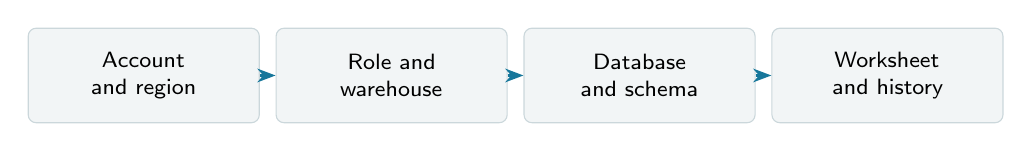
\begin{tikzpicture}[every node/.style={font=\sffamily\fontsize{8}{10}\selectfont}, b/.style={draw=thinrule,rounded corners=1mm,fill=papergray,align=center,minimum height=12mm,text width=27mm},>=Stealth]
\node[b] (a) {Account\\and region};\node[b,right=2mm of a] (b) {Role and\\warehouse};\node[b,right=2mm of b] (c) {Database\\and schema};\node[b,right=2mm of c] (d) {Worksheet\\and history};
\draw[->,thick,steelblue](a)--(b);\draw[->,thick,steelblue](b)--(c);\draw[->,thick,steelblue](c)--(d);
\end{tikzpicture}
\end{center}
{\small\color{inkgray}\textbf{Figure 3.1.} The safe inspection sequence; conceptual workflow, not a screenshot of a specific Snowsight release.}\par
\topic{3.2.2}{Worksheets and Query History}
A worksheet is useful for exploration but not sufficient as the only record of a production-minded change. Assign a descriptive title, keep commands in a companion SQL file, and run an identity/context check before making changes. Start with statements that require no warehouse execution:
\begin{lstlisting}[language=SQL,caption={Read-only session identification; actual result depends on your account.}]
SELECT CURRENT_ACCOUNT(), CURRENT_REGION(),
       CURRENT_ROLE(), CURRENT_WAREHOUSE(),
       CURRENT_DATABASE(), CURRENT_SCHEMA();
\end{lstlisting}
Query History can help identify a statement, its execution state and duration, the active warehouse and an inspectable query identifier, subject to your role and the account's retention and visibility rules. Do not treat Query History as the sole source-control or long-term audit mechanism: it cannot replace a reviewed commit, a release tag, or recorded test evidence [3].

\topic{3.2.3}{Capture evidence without leaking information}
If screenshots are needed, label them with the capture date, relevant UI version if available, role and feature context. Redact account identifiers, email addresses, customer information and tokens. Preserve \emph{what was observed} separately from \emph{what the book expects a new reader to observe}. A changed button location is a minor editorial update; a changed authorization rule is a technical correction.

\textbf{Failure mode.} A user runs \texttt{CREATE TABLE} in the wrong database because a worksheet inherited an earlier context. \textbf{Prevention:} check context and use fully qualified names in deployment scripts. \textbf{Success check:} another engineer can identify the environment and locate the SQL file that produced the worksheet result.
\repo{P023: Snowpark in Worksheets and Notebooks}{https://github.com/Snowflake-Labs/sfguide-getting-started-with-snowpark-in-worksheets-notebooks}

\newpage
% PAGE 42 / 3.3 part 1
\section*{3.3\quad Databases, schemas, tables, and warehouses}
\topic{3.3.1}{The object hierarchy and its consequences}
The chapter's demonstration uses the following nested identifiers: \texttt{BOOK\_CH03\_DEV} for the database, \texttt{LAB} for its schema, and \texttt{ENERGY\_READING} for one small table. This makes it possible to distinguish objects from session defaults. It also gives cleanup an explicit, narrow scope: remove only these objects \emph{if they were created for this lab and have no other owners or consumers}.

\begin{center}
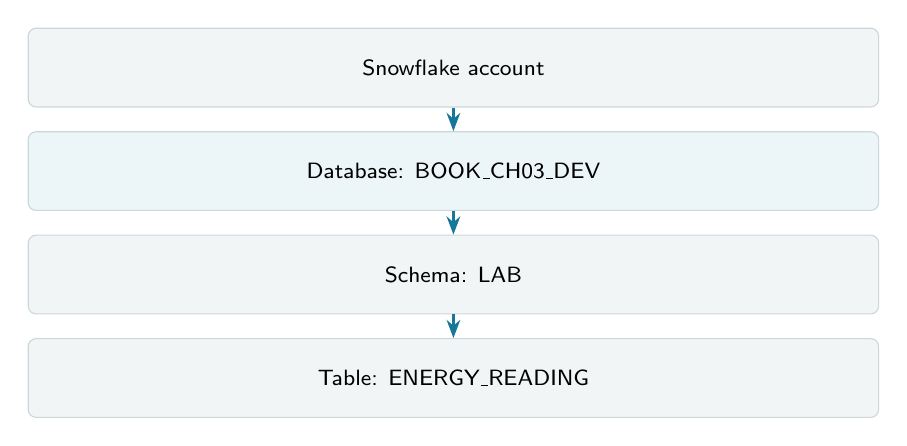
\begin{tikzpicture}[every node/.style={font=\sffamily\fontsize{8.3}{10}\selectfont}, b/.style={draw=thinrule,rounded corners=1mm,fill=papergray,align=center,minimum height=10mm},>=Stealth]
\node[b,minimum width=108mm] (a) {Snowflake account};
\node[b,below=3mm of a,minimum width=108mm,fill=lightblue] (b) {Database: BOOK\_CH03\_DEV};
\node[b,below=3mm of b,minimum width=108mm] (c) {Schema: LAB};
\node[b,below=3mm of c,minimum width=108mm] (d) {Table: ENERGY\_READING};
\draw[->,thick,steelblue](a)--(b);\draw[->,thick,steelblue](b)--(c);\draw[->,thick,steelblue](c)--(d);
\end{tikzpicture}
\end{center}
{\small\color{inkgray}\textbf{Figure 3.2.} Logical containment; the virtual warehouse is account-level compute, not a child of the database.}\par
A table is not the same thing as the warehouse that executes queries against it. Creating a database or schema is largely a metadata operation; scanning table data typically uses compute. Object creators commonly become owners, which determines who can later change objects and manage grants. The final access model must be established deliberately, not inferred from whichever administrator created the first objects [4].

\begin{lstlisting}[language=SQL,caption={DDL excerpt for a dedicated training account. Administrator review required.}]
-- Prerequisite: an approved provisioner role.
CREATE DATABASE IF NOT EXISTS BOOK_CH03_DEV;
CREATE SCHEMA IF NOT EXISTS BOOK_CH03_DEV.LAB;
CREATE TABLE IF NOT EXISTS
  BOOK_CH03_DEV.LAB.ENERGY_READING (
    OBS_ID NUMBER(38,0),
    SOURCE VARCHAR(40),
    EVENT_UTC TIMESTAMP_NTZ,
    POWER_MW FLOAT
  );
\end{lstlisting}
\textbf{Idempotency caveat.} \texttt{IF NOT EXISTS} prevents a duplicate-object error; it does not validate that an existing object's columns, owner, retention policy or grants match this lesson. Compare actual definitions before declaring the environment reproducible. A production migration system handles drift explicitly.

\newpage
% PAGE 43 / 3.3 part 2
\section*{3.3\quad Ownership, naming, and predictable context}
\topic{3.3.2}{Naming conventions and object ownership}
Names are operational controls. Prefer plain uppercase, unquoted identifiers for this lab. Use a stable purpose prefix, an environment suffix, a schema with a clear boundary, and descriptive columns with units. Avoid ambiguous names such as \texttt{DATA}, \texttt{TABLE1}, or \path{TEMP_FINAL2}. Establish consistent conventions for object name length, plurals, timestamps, and measurements. For example, \texttt{POWER\_MW} is preferable to \texttt{POWER} because it communicates the quantity and unit.

\begin{whitebox}
\textbf{Proposed naming policy}\par
Account: organization-governed and environment-specific. Database: \texttt{BOOK\_CH03\_DEV}. Schema: \texttt{LAB}. Table: \texttt{ENERGY\_READING}. Warehouse: \path{BOOK_CH03_XS}. Reader role: \texttt{BOOK\_CH03\_READER}. Query tag: \texttt{book/ch03/manual}. Every resource is disposable only when the provisioning manifest names it as such.
\end{whitebox}
Ownership should not be conflated with access to read data. A role with \texttt{OWNERSHIP} can exercise much broader control than a role with \texttt{SELECT}; an engineer who only analyzes readings should not also own the raw table. In a normal schema, the owner controls grants on objects it owns, but a managed-access schema changes who may grant privileges. Avoid universal recipes that omit schema mode or session role [4].

\textbf{Operational rule.} Use the privileged provisioning role only to establish resources. Analysts should switch to narrower reader roles for routine SQL. A separate cleanup approver should confirm which names can be dropped. This keeps administrative actions out of screenshots and tutorial examples addressed to everyday users.

\subsection*{Context inspection before every write}
The following query is a low-cost sanity check for role and namespace, but its expected output depends on the active session:
\begin{lstlisting}[language=SQL,caption={Context checkpoint for the exercise.}]
SELECT CURRENT_ROLE() AS active_role,
       CURRENT_DATABASE() AS active_db,
       CURRENT_SCHEMA() AS active_schema,
       CURRENT_WAREHOUSE() AS active_wh;
\end{lstlisting}
For an authoring workflow, add a \emph{human-readable evidence record}: date, account alias, purpose, expected role, SQL file checksum, reviewer and acceptance result. Do not store secret account credentials in the record.

\textbf{Failure mode.} \texttt{CREATE OR REPLACE TABLE} destroys an unexpectedly named object. \textbf{Safer alternative.} In instructional code use \texttt{CREATE TABLE IF NOT EXISTS} and a preflight schema check; reserve replacement for consciously reviewed migrations and test environments.
\repo{P016: Snowflake Python API Getting Started}{https://github.com/Snowflake-Labs/sfguide-getting-started-snowflake-python-api}

\newpage
% PAGE 44 / 3.3 part 3
\section*{3.3\quad Compute that stops when the experiment does}
\topic{3.3.3}{Small warehouses and auto-suspend}
A virtual warehouse executes many compute-bound SQL operations. For a short first lesson, an X-Small warehouse is an appropriate starting \emph{candidate}, not an assertion that all accounts or workloads can execute economically at that size. Configure auto-resume for convenience and auto-suspend to reduce time spent running while idle. A user-managed warehouse can still incur compute charges when it resumes, including minimum billing behavior documented for warehouse startup [5].

\begin{lstlisting}[language=SQL,caption={A bounded virtual warehouse with a suspended initial state.}]
CREATE WAREHOUSE IF NOT EXISTS BOOK_CH03_XS
  WAREHOUSE_SIZE = 'XSMALL'
  AUTO_SUSPEND = 60
  AUTO_RESUME = TRUE
  INITIALLY_SUSPENDED = TRUE
  COMMENT = 'Disposable training warehouse';
\end{lstlisting}
Never assume the command altered an existing warehouse: \texttt{IF NOT EXISTS} does not reconcile its size or suspension settings. Use \texttt{SHOW WAREHOUSES} and inspect the matching resource settings. If an existing warehouse does not match, obtain approval before changing it. If the training account provides a managed shared warehouse, reuse it instead of allocating an additional one.

\begin{center}
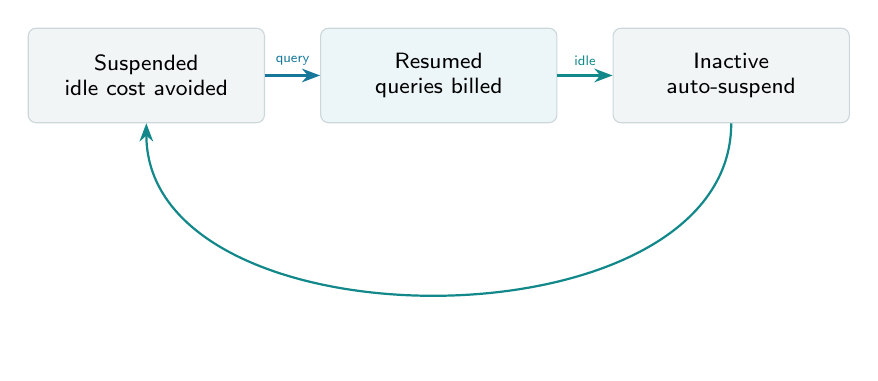
\begin{tikzpicture}[every node/.style={font=\sffamily\fontsize{8}{9}\selectfont}, b/.style={draw=thinrule,fill=papergray,rounded corners=1mm,minimum width=30mm,minimum height=12mm,align=center},>=Stealth]
\node[b] (a) {Suspended\\ idle cost avoided};\node[b,right=7mm of a,fill=lightblue] (b) {Resumed\\ queries billed};\node[b,right=7mm of b] (c) {Inactive\\ auto-suspend};
\draw[->,thick,steelblue] (a)--node[above,font=\sffamily\tiny]{query}(b);
\draw[->,thick,teal] (b)--node[above,font=\sffamily\tiny]{idle}(c);
\draw[->,thick,teal] (c.south) to[out=-90,in=-90] (a.south);
\end{tikzpicture}
\end{center}
{\small\color{inkgray}\textbf{Figure 3.3.} Warehouse lifecycle; conceptual only. Compute stop does not suspend independent serverless services or remove stored objects.}\par
\textbf{Risk check.} A warehouse with \texttt{AUTO\_SUSPEND=0} may remain active indefinitely; a training resource should not be configured this way without explicit justification. A 60-second auto-suspend does not mean a one-second query always costs one second. Billing, caching, and background service cost require separate inspection.

\begin{insight}
\textbf{Performance is not the first success criterion}\par
This chapter's success is a known role, known cost control, repeatable table definition and safe cleanup. Later chapters will investigate Query Profile, ELT execution and performance using real measurements.
\end{insight}
\textbf{Evidence:} size, suspension settings, administrator approval.
\repo{P016: Provisioning Objects with the Python API}{https://github.com/Snowflake-Labs/sfguide-getting-started-snowflake-python-api}

\newpage
% PAGE 45 / 3.4
\section*{3.4\quad Users, roles, and basic grants}
\topic{3.4.1}{Role-based access and the grant chain}
Snowflake access control separates a \emph{user identity} from a \emph{role} that carries privileges. A typical reader needs \texttt{USAGE} on the compute warehouse and the appropriate containing database and schema, plus \texttt{SELECT} on the table. A privilege on the warehouse alone does not authorize data access. Conversely, having table \texttt{SELECT} without available compute is generally insufficient to run a scan [4].

\begin{center}
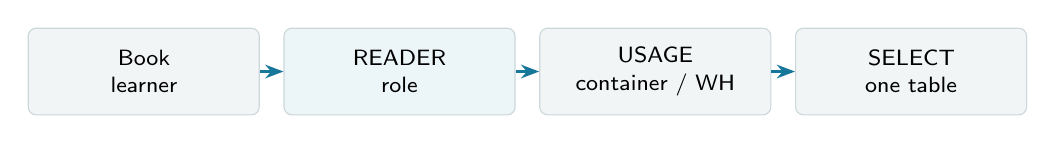
\begin{tikzpicture}[every node/.style={font=\sffamily\fontsize{8}{9.8}\selectfont}, b/.style={draw=thinrule,rounded corners=1mm,fill=papergray,minimum height=11mm,text width=27mm,align=center},>=Stealth]
\node[b] (u) {Book\\learner};\node[b,right=3mm of u,fill=lightblue] (r) {READER\\role};\node[b,right=3mm of r] (g) {USAGE\\container / WH};\node[b,right=3mm of g] (s) {SELECT\\one table};
\draw[->,thick,steelblue](u)--(r);\draw[->,thick,steelblue](r)--(g);\draw[->,thick,steelblue](g)--(s);
\end{tikzpicture}
\end{center}
{\small\color{inkgray}\textbf{Figure 3.4.} A least-privilege reader path; arrows express the teaching concept, not a literal internal authorization sequence.}\par
\topic{3.4.2}{Execution roles versus ownership roles}
Separate \emph{provisioner}, \emph{reader}, and any future \emph{writer} permissions. An approved security administrator can create the reader role; an authorized object owner or grant manager can assign object privileges. The grant sequence below is a \emph{provisioning example}, not SQL for unprivileged users to run. Role assignment to named users must follow an identity review.
\begin{lstlisting}[language=SQL,caption={Administrator-authorized role and object grants.}]
-- Security administrator or approved delegate:
CREATE ROLE IF NOT EXISTS BOOK_CH03_READER;
-- Authorized grant manager, after lab objects exist:
GRANT USAGE ON WAREHOUSE BOOK_CH03_XS
  TO ROLE BOOK_CH03_READER;
GRANT USAGE ON DATABASE BOOK_CH03_DEV
  TO ROLE BOOK_CH03_READER;
GRANT USAGE ON SCHEMA BOOK_CH03_DEV.LAB
  TO ROLE BOOK_CH03_READER;
GRANT SELECT ON TABLE
  BOOK_CH03_DEV.LAB.ENERGY_READING
  TO ROLE BOOK_CH03_READER;
\end{lstlisting}
\topic{3.4.3}{Negative tests matter}
With the reader role active and assigned, the learner must be able to \texttt{SELECT} from the sample table but should \emph{not} be able to \texttt{INSERT} into it or create new tables. Use a read-only negative test when possible, such as checking documented grants; a deliberately denied \texttt{CREATE TABLE} should be executed only in an isolated sandbox after approval. \textbf{Do not} use \texttt{ACCOUNTADMIN} to ``fix'' a missing student permission.

A role can inherit privileges from other assigned roles, and secondary role behavior can affect access. Before interpreting a successful negative test, capture the primary and any active secondary roles. An expected denial is useful evidence only when the intended identity context is known.
\repo{P024: Terraform Snowflake RBAC Infrastructure}{https://github.com/Infostrux-Solutions/terraform-snowflake-rbac-infra}

\newpage
% PAGE 46 / 3.5.1
\section*{3.5\quad SQL worksheets, Snowflake CLI, and Git}
\topic{3.5.1}{Worksheets for exploration; files for the durable record}
Worksheets lower the barrier to investigating a table, testing a \texttt{WHERE} clause or evaluating a \texttt{CREATE} statement. Their weakness is not their interface; it is the temptation to let the worksheet become the only source of truth. A colleague cannot review a reproducible deployment from a screenshot of a successful command. The book therefore stores the \emph{same SQL} in named files, with comments explaining prerequisites and acceptance criteria.

A useful working directory is:
\begin{lstlisting}[caption={Proposed Chapter 3 companion-lab repository.}]
chapter03-environment/
  README.md
  sql/
    01_bootstrap.sql
    02_grants.sql
    03_verify.sql
    99_cleanup.sql
  python/connection_probe.py
  .env.example
  .gitignore
  evidence/   # no credentials / private screenshots
\end{lstlisting}
\textbf{Make execution explicit.} A file that creates a database is not safe to run under every role or account. Each SQL file should declare its intended environment, approval authority, expected object names, impact, rollback procedure and related documentation. Keep identity-specific overrides out of version control.

\begin{whitebox}
\textbf{A reviewable change, not merely an executed change}\par
\path{01_bootstrap.sql} defines the lab resources. \path{02_grants.sql} is reviewed by an access administrator. \path{03_verify.sql} asserts the intended role and data visibility. \path{99_cleanup.sql} removes only named resources after a separate approval check. Evidence records both the script revision and observed results.
\end{whitebox}
\textbf{Version the interpretation.} If a lab step works today but fails next year because a CLI option has changed, a source-control tag and documented tool version make the discrepancy diagnosable. Update the book's \emph{companion release}, not silently overwrite an old edition with a new command. The history is part of the educational value.

\textbf{Failure mode.} A worksheet contains both exploratory cleanup and a valid production query; exporting and executing everything as one file damages unrelated objects. \textbf{Prevention:} separate read-only verification, controlled provisioning and destructive teardown into distinct reviewed files.

\repo{P025: Official Snowflake CLI Templates}{https://github.com/snowflakedb/snowflake-cli-templates}

\newpage
% PAGE 47 / 3.5.2
\section*{3.5\quad A secure CLI workflow}
\topic{3.5.2}{Configuring Snowflake CLI}
Snowflake CLI provides a local \texttt{snow} command for testing a connection and executing SQL files. It is a client, not an extra data warehouse. Start with the officially maintained CLI installation instructions appropriate to your operating system and record the installed version. The current documentation describes configuration in \texttt{config.toml} and, for shared developer-tool connections, \texttt{connections.toml}; parameters may be overridden by the environment [6].

For a human using organizational single sign-on, a connection with an external-browser authenticator may be appropriate \emph{if supported by the identity policy}. A local configuration example \emph{without secrets} is:
\begin{lstlisting}[caption={Illustrative CLI config.toml; adapt account and user locally.}]
[connections.book_dev]
account = "your_org-your_account"
user = "your_login"
authenticator = "EXTERNALBROWSER"
role = "BOOK_CH03_READER"
warehouse = "BOOK_CH03_XS"
database = "BOOK_CH03_DEV"
schema = "LAB"
\end{lstlisting}
Do not commit a \texttt{config.toml} containing session tokens, password fields or locally identifying connection information to a public repository. Protect the configuration file's filesystem permissions. Automated CI usually requires a different, explicitly authorized noninteractive authentication method (for example, managed federation or a protected key), with its privileges no broader than the job requires [6].

\begin{lstlisting}[caption={Documented CLI command forms; requires approved account access.}]
snow --version
snow connection test --connection book_dev
snow sql --connection book_dev \
  --query "SELECT CURRENT_ROLE()"
snow sql --connection book_dev \
  --filename sql/03_verify.sql
\end{lstlisting}
The first line runs locally. The remaining lines contact Snowflake and may open browser authentication or resume compute for certain statements. Do not interpret a connection test as proof that permissions for every chapter exercise are correct: authentication and access to a specific table are separate claims.

\textbf{Common failure patterns:} wrong organization-account identifier; incorrect connection name; token/MFA problems; nonexistent default database; role not granted to the identity; warehouse privileges missing. Diagnose with recorded error category and session context, not by putting secrets in a screenshot. \textbf{Success check:} CLI authentication works and \texttt{CURRENT\_ROLE()} reports the expected least-privileged role.
\repo{P026: Official Snowflake CLI Action}{https://github.com/snowflakedb/snowflake-cli-action}

\newpage
% PAGE 48 / 3.5.3
\section*{3.5\quad Version control and delivery boundaries}
\topic{3.5.3}{Git changes, code review, and pull requests}
The purpose of Git is to make the \emph{definition} of the environment reviewable. Give one pull request a narrow scope: ``introduce Chapter 3 DEV bootstrap,'' not ``fix all Snowflake settings.'' The change includes tests, explanations, cleanup criteria and a manifest of the resources the scripts will affect. Reviewers should be able to reject a grant that gives inappropriate ownership without needing a live account to spot the error.

\begin{center}
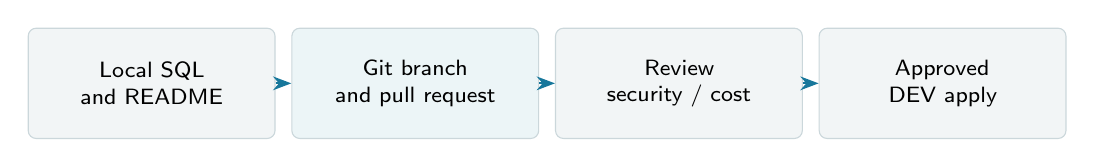
\begin{tikzpicture}[every node/.style={font=\sffamily\fontsize{8}{9.5}\selectfont}, b/.style={draw=thinrule,rounded corners=1mm,fill=papergray,text width=29mm,minimum height=14mm,align=center},>=Stealth]
\node[b] (a) {Local SQL\\and README};\node[b,right=2mm of a,fill=lightblue] (b) {Git branch\\and pull request};\node[b,right=2mm of b] (c) {Review\\security / cost};\node[b,right=2mm of c] (d) {Approved\\DEV apply};
\draw[->,thick,steelblue](a)--(b);\draw[->,thick,steelblue](b)--(c);\draw[->,thick,steelblue](c)--(d);
\end{tikzpicture}
\end{center}
{\small\color{inkgray}\textbf{Figure 3.5.} Suggested change-control sequence. Automated deployment is an optional advanced step, not part of this chapter's required lab.}\par
\textbf{Review checklist for a pull request:}
\begin{itemize}
\item Resource names are scoped to \texttt{BOOK\_CH03\_DEV}; no production defaults appear.
\item Code has explicit prerequisite roles, effects, and expected verification output.
\item No live secret, private key, access token, customer data, or account URL is committed.
\item An authorized reviewer approves grants and cost-bearing resource creation.
\item Cleanup names exact resources and refuses ambiguous or shared-object deletion.
\item A passing check refers to the submitted commit, not an earlier local file.
\end{itemize}
Continuous integration can lint SQL, validate file encoding and check for accidentally committed secrets \emph{without} deploying any Snowflake resources. A separate restricted workflow may later perform tests in a dedicated account. Treating GitHub Actions as an administrator by default is a security anti-pattern: runner compromise would otherwise become cloud-administration compromise.

\begin{insight}
\textbf{A release is reproducible when its identity is known}\par
Record the book edition, repository URL, version tag, relevant package versions, and tested commit SHA. A screenshot of a green build indicator without the commit and execution context is weak evidence.
\end{insight}
\textbf{Failure mode.} A maintainer merges an unreviewed \texttt{GRANT OWNERSHIP} because the script happens to be in a repository. \textbf{Decision rule:} separate code review, privilege approval and deployment authority. These may be performed by different people even in a small team.
\repo{P026: Snowflake CLI CI action}{https://github.com/snowflakedb/snowflake-cli-action}

\newpage
% PAGE 49 / 3.6 part 1
\section*{3.6\quad Connecting Python and SQL tools}
\topic{3.6.1}{Python Connector and connection verification}
Python is useful when an ingestion job must call an API, validate a file or schedule a query. Snowflake provides an official Python Connector; a successful connection establishes a session, not a proof that a pipeline's transformations are correct. Install the connector in an isolated environment and pin a version in the companion project after testing [7].

\begin{lstlisting}[language=Python,caption={Short connection-probe pattern; no embedded password.}]
import os
import snowflake.connector

with snowflake.connector.connect(
    account=os.environ["SNOWFLAKE_ACCOUNT"],
    user=os.environ["SNOWFLAKE_USER"],
    authenticator="externalbrowser",
    role="BOOK_CH03_READER",
    warehouse="BOOK_CH03_XS",
    database="BOOK_CH03_DEV",
    schema="LAB",
) as conn:
    with conn.cursor() as cur:
        cur.execute("SELECT CURRENT_ROLE(), CURRENT_REGION()")
        print(cur.fetchone())  # expected: role and account region
\end{lstlisting}
This example targets a \emph{human interactive} development session in an environment where external-browser sign-in is configured. Do not use it as the default for unattended automation; interactive login can block a headless process. The project also supplies an offline Python preflight checker that validates file and environment conventions without opening a cloud connection.

\textbf{Error taxonomy.} Distinguish DNS/network failures, authentication failures, unauthorized roles, suspended or unauthorized warehouse access, nonexistent objects, SQL compilation errors, and queries that run but return wrong values. Changing one category's configuration cannot be assumed to repair another.

\begin{whitebox}
\textbf{No confirmed live test}\par
The connector snippet is based on documented API patterns. This manuscript has not authenticated to the reader's Snowflake account; it therefore gives \emph{expected session fields}, not invented query identifiers, timings, or copied UI results.
\end{whitebox}
\textbf{Evidence to capture:} Python version, connector version, the selected connection mode, the active role and successful clean connection closure. If the account employs MFA or federation policy, follow the approved identity guidance rather than bypassing security requirements.
\repo{P027: Official Snowflake Python Connector}{https://github.com/snowflakedb/snowflake-connector-python}

\newpage
% PAGE 50 / 3.6 part 2
\section*{3.6\quad Secrets and the session lifecycle}
\topic{3.6.2}{Secret storage and environment variables}
Do not put credentials in SQL text, book screenshots or \texttt{.env.example}. Environment variables are convenient for a developer but are not an encryption scheme: operating-system processes, diagnostic reports or improperly configured CI logs can still expose them. Use a managed secret store or an approved authentication flow for real deployments. In Git, ignore local secret files; examine prior commits because deleting a leaked key from the newest revision does not revoke it.

\begin{lstlisting}[caption={Committable .env.example: values deliberately left blank.}]
SNOWFLAKE_ACCOUNT=
SNOWFLAKE_USER=
SNOWFLAKE_ROLE=BOOK_CH03_READER
SNOWFLAKE_WAREHOUSE=BOOK_CH03_XS
SNOWFLAKE_DATABASE=BOOK_CH03_DEV
SNOWFLAKE_SCHEMA=LAB
\end{lstlisting}
Threat model: committed secrets, leaked log output, and excessive privileges. Rotate any exposed credential; erasing a public example does not revoke it.

\topic{3.6.3}{Controlled lifecycle and clean exit}
Open a connection only when needed, close it after failure, and understand transaction boundaries. For this chapter's \texttt{SELECT}, no rollback is required. Ingestion writes in later chapters need retry-safe behavior.

\textbf{Distinguish three kinds of termination:}
\begin{enumerate}
\item \emph{Client closure} ends the Python session or cursor. It is not an account deletion action.
\item \emph{Warehouse suspension} stops eligible user-managed compute. It does not delete tables or terminate every serverless service.
\item \emph{Lab teardown} explicitly removes authorized disposable objects after validation and handover.
\end{enumerate}
\begin{insight}
\textbf{Decision: interactive versus machine identity}\par
Choose interactive SSO for an identified human if organization policy permits; choose federation or another approved machine-to-machine method for scheduled pipelines. Static password-in-code is not an acceptable shortcut for either mode.
\end{insight}
\textbf{Failure mode.} A Python task returns correct results but hangs in a container because the authenticator tries to open a browser. \textbf{Response:} change the authentication architecture through the identity administrator, not by switching to an unprotected plaintext password.

\textbf{Checkpoint.} Document the identity, secret source, exit path and effective role [7].
\repo{P027: Snowflake Python Connector}{https://github.com/snowflakedb/snowflake-connector-python}

\newpage
% PAGE 51 / 3.7
\section*{3.7\quad Naming and DEV/TEST/PROD boundaries}
\topic{3.7.1}{Object naming as an operational signal}
A well-named object makes its environment and intended owner visible. The convention \texttt{BOOK\_CH03\_DEV.LAB.ENERGY\_READING} tells a reviewer substantially more than \texttt{DATA.PUBLIC.T1}. Naming does not confer security, yet it supports automated checks and reduces human error. Use uppercase unquoted names for this training environment; do not quietly introduce case-sensitive quoted names in the next migration.

\topic{3.7.2}{Separating development, testing, and production}
\emph{Development} is a place to change code and inspect experiments. \emph{Testing} is a place to evaluate a reviewed artifact against representative, controlled data. \emph{Production} serves real users under availability, access and change-control obligations. Three schemas with different prefixes inside one administrator-owned account are \emph{not equivalent} to three isolated accounts. Choose boundaries based on impact, organization scale, data sensitivity and cost.

\begin{center}
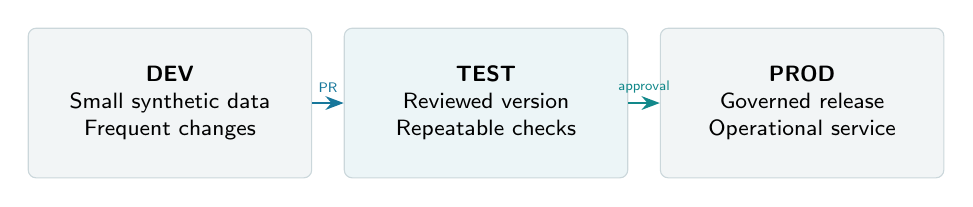
\begin{tikzpicture}[every node/.style={font=\sffamily\fontsize{8}{9.7}\selectfont}, b/.style={draw=thinrule,rounded corners=1mm,fill=papergray,minimum width=36mm,minimum height=19mm,align=center},>=Stealth]
\node[b] (d) {\textbf{DEV}\\ Small synthetic data\\ Frequent changes};
\node[b,right=4mm of d,fill=lightblue] (t) {\textbf{TEST}\\ Reviewed version\\ Repeatable checks};
\node[b,right=4mm of t] (p) {\textbf{PROD}\\ Governed release\\ Operational service};
\draw[->,thick,steelblue](d)--node[above,font=\sffamily\tiny]{PR}(t);
\draw[->,thick,teal](t)--node[above,font=\sffamily\tiny]{approval}(p);
\end{tikzpicture}
\end{center}
{\small\color{inkgray}\textbf{Figure 3.6.} Promotion of an artifact, not blind copying of development data into production.}\par
\topic{3.7.3}{Preventing accidental production operations}
Three safeguards complement one another: a context guard in deployment scripts, policy-based authorization that rejects unauthorized actions, and a human-reviewed deployment gate. A guard alone is insufficient if the same service account holds \texttt{ACCOUNTADMIN}. Avoid production credentials in local notebooks. Require separate identities or permissions for production changes, and require explicit approval for destructive migrations.

\begin{lstlisting}[language=SQL,caption={A safe, read-only preflight query; check results before running DDL.}]
SELECT CURRENT_ACCOUNT() AS account_id,
       CURRENT_ROLE() AS active_role,
       CURRENT_DATABASE() AS database_name,
       CURRENT_WAREHOUSE() AS warehouse_name;
\end{lstlisting}
\textbf{Common error.} The deployment succeeded against the wrong account because both environments used identically named schemas. \textbf{Remedy.} Pin and report the account identity in the pipeline configuration; make the deployment stop if it differs from the approved target. Exclude secrets from the resulting log. More complete delivery and rollback patterns appear in Chapter 10.
\repo{P028: Snowflake DevOps Quickstart}{https://github.com/Snowflake-Labs/sfguide-getting-started-with-snowflake-devops}
\repo{P029: Snowflake Terraform CI/CD Demo}{https://github.com/sfc-gh-sekim/cicd-snowflake-with-terraform-demo}

\newpage
% PAGE 52 / 3.8.1
\section*{3.8\quad Budgets, resource monitors, and cost guardrails}
\topic{3.8.1}{Budgets and supported cost monitoring}
A Snowflake \emph{Budget} monitors projected credit usage for supported compute consumption and sends notifications when projected use exceeds a configured monthly limit. Account-level and custom budgets have different scopes; supported service types, AI charges, and additional budget behavior may change over time [8]. A budget is primarily \emph{visibility and notification}, not an automatic universal suspension switch.

\begin{whitebox}
\textbf{Billing vocabulary to keep separate}\par
\emph{Credit consumption} measures certain compute usage. \emph{Monetary cost} depends on the contract, region, edition and other charges. \emph{Budget threshold} is a monitoring target. \emph{Resource-monitor quota} is a limit configured for assigned user-managed warehouses. These quantities must never be treated as identical in a book's worked example.
\end{whitebox}
Budgets can themselves generate small serverless measurement and metadata costs. Credit data may not update instantaneously. Do not present an alert screenshot as proof that all current costs have been captured, or assume a notification will be received if no valid alert delivery channel has been set up [8].

\begin{center}
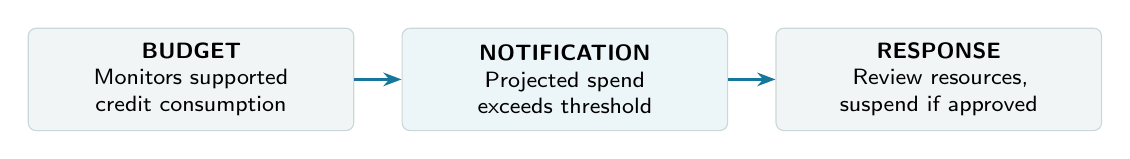
\begin{tikzpicture}[every node/.style={font=\sffamily\fontsize{8}{9.6}\selectfont}, b/.style={draw=thinrule,fill=papergray,rounded corners=1mm,minimum height=13mm,text width=39mm,align=center},>=Stealth]
\node[b] (b) {\textbf{BUDGET}\\Monitors supported\\credit consumption};
\node[b,right=6mm of b,fill=lightblue] (n) {\textbf{NOTIFICATION}\\Projected spend\\exceeds threshold};
\node[b,right=6mm of n] (r) {\textbf{RESPONSE}\\Review resources,\\suspend if approved};
\draw[->,thick,steelblue](b)--(n);\draw[->,thick,steelblue](n)--(r);
\end{tikzpicture}
\end{center}
{\small\color{inkgray}\textbf{Figure 3.7.} Budget response model. No automatic universal charge-stop is implied.}\par
For our demonstration, the recommended order is: ask an account administrator whether a budget already exists; request an appropriate warning threshold; set notification recipients; and confirm which services the budget covers. Do not activate chargeable features just to obtain a screenshot for the book. A trial account may have its own separate balance controls.

\textbf{Failure mode.} A learner believes ``the budget is set to five credits, so the account cannot spend six.'' This is false: a threshold notification is not a hard spending cap. \textbf{Decision checkpoint:} who responds to the warning, and what will they stop first? Document a named owner and escalation path.
\repo{P030: Snowflake Usage App}{https://github.com/streamlit/snowflake-usage-app}

\newpage
% PAGE 53 / 3.8.2--3
\section*{3.8\quad Controls that can interrupt a warehouse}
\topic{3.8.2}{Resource Monitor scope and suspension actions}
A Resource Monitor tracks credit usage of \emph{user-managed virtual warehouses} assigned to it. It can notify and, at a threshold, suspend assigned warehouses. It does \emph{not} cover every serverless or AI workload and cannot replace a full account cost strategy [8,9]. A monitor can use a recurring quota period; resets and notification timing should be checked against current documentation. Use dedicated monitor objects only with administrative approval.

\begin{lstlisting}[language=SQL,caption={OPTIONAL admin-only Resource Monitor configuration; not executed.}]
CREATE RESOURCE MONITOR BOOK_CH03_MONITOR
  WITH CREDIT_QUOTA = 5
  FREQUENCY = MONTHLY
  TRIGGERS
    ON 50 PERCENT DO NOTIFY
    ON 100 PERCENT DO SUSPEND;
-- Assigned by an authorized warehouse admin:
ALTER WAREHOUSE BOOK_CH03_XS
  SET RESOURCE_MONITOR = BOOK_CH03_MONITOR;
\end{lstlisting}
This is an \emph{illustrative configuration}, not a guarantee of five credits as a total account cap. \texttt{SUSPEND} normally lets running queries complete; \texttt{SUSPEND\_IMMEDIATE} has a stronger interruption effect and needs particular care. Only approved administrators should create monitors or change warehouse assignments; these actions might affect teammates if the warehouse is shared [9].

\topic{3.8.3}{Cost response and emergency-stop runbook}
\textbf{Before:} check ownership, auto-suspend, budget and service scope. \textbf{During:} stop unexpected retries. \textbf{After:} suspend dedicated compute and inspect remaining objects.

\begin{lstlisting}[language=SQL,caption={Approved stop action; only use against a dedicated lab warehouse.}]
ALTER WAREHOUSE BOOK_CH03_XS SUSPEND;
SHOW WAREHOUSES LIKE 'BOOK_CH03_XS';
\end{lstlisting}
Do not suspend a shared production warehouse to complete a book exercise. Suspending the warehouse can prevent new user-managed SQL work, but it cannot be treated as an account-wide freeze; some consumption continues independently. If the account is unexpectedly billed, escalate to its administrator and billing owner.

\begin{insight}
\textbf{An accurate rule of thumb}\par
Use \emph{budgets} to discover and be warned about supported credit use; use \emph{resource monitors} when warehouse-level suspension is required; use least privilege, guardrails and human response for the remaining risks.
\end{insight}
\textbf{Check:} warehouse suspension cannot cap all serverless or AI costs.
\repo{P031: dbt Snowflake Monitoring}{https://github.com/get-select/dbt-snowflake-monitoring}

\newpage
% PAGE 54 / 3.9
\section*{3.9\quad Reusable environment bootstrap scripts}
\topic{3.9.1}{Idempotent DDL---and what it does not guarantee}
A bootstrap should create the same \emph{intended} lab resources on repeat execution, report whether they already existed and refuse to modify shared objects silently. Simple \texttt{IF NOT EXISTS} clauses reduce accidental duplicate creation but do not reconcile column types, warehouse settings or ownership. A robust workflow therefore has a \emph{preflight}, a \emph{controlled apply}, \emph{verification} and \emph{cleanup}. In production, schema migrations and infrastructure-as-code tools extend this pattern with state, drift detection and review [10].

\begin{center}
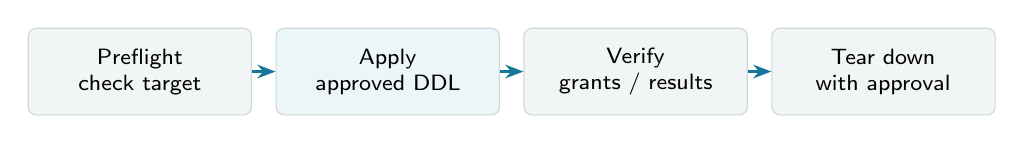
\begin{tikzpicture}[every node/.style={font=\sffamily\fontsize{8}{9.4}\selectfont}, b/.style={draw=thinrule,rounded corners=1mm,fill=papergray,text width=26mm,minimum height=11mm,align=center},>=Stealth]
\node[b] (a) {Preflight\\check target};\node[b,right=3mm of a,fill=lightblue] (b) {Apply\\approved DDL};\node[b,right=3mm of b] (c) {Verify\\grants / results};\node[b,right=3mm of c] (d) {Tear down\\with approval};
\draw[->,thick,steelblue](a)--(b);\draw[->,thick,steelblue](b)--(c);\draw[->,thick,steelblue](c)--(d);
\end{tikzpicture}
\end{center}
{\small\color{inkgray}\textbf{Figure 3.8.} Four stages of a repeatable lab, with separate administrative permissions.}\par
\topic{3.9.2}{Parameterization and environment files}
A reusable script should not depend on undocumented local worksheet defaults. Use fully qualified objects or explicitly set the context, and keep account identifiers and authentication settings in protected local configuration. An \texttt{.env.example} can enumerate required variable names without publishing values. A deployment tool may substitute validated environment identifiers, but never template arbitrary user strings into privileged SQL object names without validation.

\topic{3.9.3}{Safe teardown and audit trail}
Destructive cleanup is a deployment, not housekeeping. Require a written manifest of lab-owned resources, a confirmation that no other consumers depend on them, and a verified account/role check. \texttt{DROP DATABASE} removes an entire hierarchy, so the sample cleanup file defaults to individually removing its \emph{named table and schema} only after authorization. It leaves the database and roles untouched for a responsible administrator to review. The resource monitor and warehouse likewise require ownership checks before deletion.

\begin{whitebox}
\textbf{Definition of a reproducible first environment}\par
A peer can read the manifest, verify permissions, provision isolated objects, use a reader role successfully, observe an expected denial for an unauthorized operation, stop compute, and identify precisely which resources remain. Every step has a documented stop condition and an owner.
\end{whitebox}
\textbf{Failure mode.} A cleanup script deletes \texttt{BOOK\_CH03\_DEV} even though another chapter's dataset has been added. \textbf{Prevention:} treat the original lab manifest as a whitelist and refuse broad deletion when objects have drifted.
\repo{P032: Terraform Sample}{https://github.com/Snowflake-Labs/sfguide-terraform-sample}
\repo{P033: Official Terraform Provider}{https://github.com/snowflakedb/terraform-provider-snowflake}

\newpage
% PAGE 55 / Lab part 1
\section*{3.L\quad Guided lab: a governed first workspace}
\topic{3.L.1}{Prerequisites, permissions, and cost boundary}
\textbf{Goal.} In a dedicated test account, define a small database and sample table, grant a read-only role, and show that the role cannot write. Use the \emph{offline track} first if you do not have authorized cloud access. No step asks for a real customer dataset. The synthetic readings below are demonstrative only and do not claim to describe Finland's actual electricity production.

\textbf{Preparation:} (a) record the selected account and role; (b) obtain a provisioning approval; (c) choose X-Small or reuse an approved suspended warehouse; (d) enable an available monitoring/alert plan; (e) keep a 10-minute time box; (f) open the companion scripts and verify that all object names start with \texttt{BOOK\_CH03}. Restrict roles and grants to the training account.

\topic{3.L.2}{Create, observe, and validate}
Provisioning uses separate files: \path{01_bootstrap.sql} for objects, \path{02_grants.sql} for administrator-reviewed access, and \path{03_verify.sql} for the reader. Do not combine them into an unrestricted student deployment.

\begin{lstlisting}[language=SQL,caption={Selected rows from the standalone bootstrap lab; educational values only.}]
-- Run only after administrator authorization.
INSERT INTO BOOK_CH03_DEV.LAB.ENERGY_READING
  (OBS_ID, SOURCE, EVENT_UTC, POWER_MW)
SELECT 1, 'synthetic_wind',
       '2026-01-15 12:00:00'::TIMESTAMP_NTZ, 82.0
WHERE NOT EXISTS (
  SELECT 1 FROM BOOK_CH03_DEV.LAB.ENERGY_READING
  WHERE OBS_ID = 1);
\end{lstlisting}
The conditional insertion makes this \emph{small example} reasonably repeatable, but it is not a general exactly-once ingestion protocol. The subsequent check deliberately specifies the table's namespace and verifies the intended role. \emph{Expected}, not observed, read-only output for the one synthetic row: a row count of one, \texttt{SOURCE='synthetic\_wind'}, and \texttt{POWER\_MW=82.0}; these values are examples only.

\begin{lstlisting}[language=SQL,caption={Read-only verification excerpt.}]
SELECT CURRENT_ROLE() AS role_name;
SELECT COUNT(*) AS row_count,
       MIN(POWER_MW) AS min_power_mw
FROM BOOK_CH03_DEV.LAB.ENERGY_READING;
\end{lstlisting}
\textbf{Negative access test.} After approval, run \path{04_negative_test.sql} with only the reader role. The write should fail. Record the redacted error and stop if the write succeeds.

\textbf{Offline:} \path{python lab_preflight.py} checks files and names, not cloud behavior.

\newpage
% PAGE 56 / Lab part 2 and references
\section*{3.L\quad Evidence, cleanup, and review}
\topic{3.L.3}{What success looks like---and how to recover}
A passing cloud session demonstrates \emph{four separate facts}: the authorized provisioner created expected objects; the reader can query the one synthetic row; the unauthorized write test is denied; and the assigned warehouse can be suspended by its authorized operator. A successful offline checker demonstrates \emph{only} syntactic preflight properties. If permissions fail, inspect grants and secondary roles. If objects differ from the manifest, stop; do not overwrite them in place. If any billing warning appears, suspend dedicated compute and escalate.

\textbf{Cleanup.} Stop clients; inspect named objects, dependencies and the active account; apply \path{99_cleanup.sql} only to the authorized disposable table. The script intentionally leaves the database, warehouse, roles and monitor for an administrator to review. Record remaining objects and their owner. A clean \emph{exit} is not necessarily a blank account.

\topic{3.L.4}{Exercises and a scored acceptance rubric}
\begin{enumerate}
\item \textbf{Foundation:} describe the account/database/schema/warehouse hierarchy and name two reasons a schema prefix is not a substitute for account separation.
\item \textbf{Applied:} adapt the read-only verification for a second synthetic energy source and explain how to avoid duplicating its seed row.
\item \textbf{Architecture decision:} an analyst requests permanent \texttt{ACCOUNTADMIN} to simplify development. Design a narrower role and list the grants it needs.
\item \textbf{Cost incident:} a scheduled job keeps running after the warehouse is suspended. Name two possible causes and two distinct controls to investigate.
\end{enumerate}
\textbf{Rubric (10 points):} identity/namespace correctness (2); least privilege and denied write (3); resource and budget scope explained accurately (2); versioned reproducibility evidence (2); safe cleanup decision (1). \emph{Passing standard:} at least 8 points with no unauthorized access or destructive-change failure.

\begin{insight}
\textbf{Chapter takeaway}\par
The first secure environment is not the one with the most services enabled. It is the one whose identity, objects, grants, cost exposure, evidence and teardown are explicit. Chapter 4 will use this boundary to build testable SQL models instead of relying on an unreviewed worksheet.
\end{insight}
{\sffamily\bfseries\fontsize{9}{11}\selectfont References and further reading}\par
{\fontsize{8.1}{9.5}\selectfont\color{inkgray}
[1] Snowflake: \href{https://docs.snowflake.com/en/user-guide/admin-account-identifier}{Account identifiers}.\quad [2] Snowflake: \href{https://docs.snowflake.com/en/user-guide/admin-trial-account}{Trial accounts}.\quad [3] Snowflake: \href{https://docs.snowflake.com/en/user-guide/ui-snowsight}{Snowsight}.\quad [4] Snowflake: \href{https://docs.snowflake.com/en/user-guide/security-access-control-overview}{Access control}.\quad [5] Snowflake: \href{https://docs.snowflake.com/en/sql-reference/sql/create-warehouse}{CREATE WAREHOUSE}.\quad [6] Snowflake: \href{https://docs.snowflake.com/en/developer-guide/snowflake-cli/connecting/configure-connections}{CLI connections}.\quad [7] Snowflake: \href{https://docs.snowflake.com/en/developer-guide/python-connector/python-connector-connect}{Python Connector}.\quad [8] Snowflake: \href{https://docs.snowflake.com/en/user-guide/cost-controlling}{Controlling cost}.\quad [9] Snowflake: \href{https://docs.snowflake.com/en/sql-reference/sql/create-resource-monitor}{CREATE RESOURCE MONITOR}.\quad [10] Snowflake: \href{https://github.com/snowflakedb/terraform-provider-snowflake}{Terraform provider}.\quad \par}
\end{document}
